\documentclass{article}
\usepackage{pgfplots}
\usepgfplotslibrary{fillbetween}

\pgfplotsset{compat=1.10}
\pgfmathsetseed{42}
\begin{document}
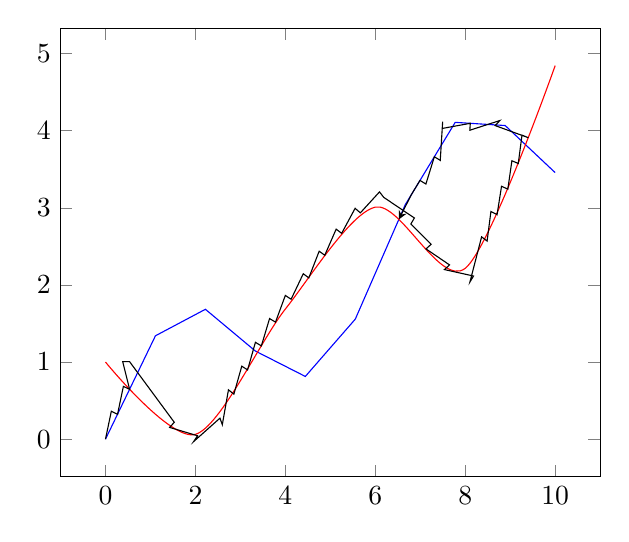
\begin{tikzpicture}
\begin{axis}[domain=0:10,samples=10]
\addplot[name path=first,blue]
    {sin(deg(x)) + 2/5*x};
\addplot[name path=second,red,
    samples=6,smooth]
    {cos(deg(1.2*x)) + 2/5*x};
\draw[black,-stealth,
    decorate,decoration={
        saw,
        post=lineto,
        post length=10pt},
    intersection segments={
        of=first and second,
        sequence={L1 -- R2 -- R3
            -- R4 -- L-2[reverse]}
    },
];
\end{axis}
\end{tikzpicture}


\pgfdeclarelayer{pre main}
\begin{tikzpicture}
    \pgfsetlayers{pre main,main}
    \draw[-stealth,thick,name path=A,red]
    (0,0) -- (1,1);
    \draw[-stealth,thick,name path=B,blue]
    (0,1) -- (1,0);
    \pgfonlayer{pre main}
    \draw[
        green,
        line width=2pt,
        intersection segments={
            of=A and B,
            sequence={L{-1} R*[reverse]}}];
    \endpgfonlayer
\end{tikzpicture}

\end{document}

